\documentclass{beamer}

\usepackage{graphicx}
\usepackage{courier}
\usepackage{xcolor}

\title{Outline of some new features for SHOP}
\subtitle{ECCC,CMC,CMDE}
\author{Luis Morales, Dorothy Dunford}

\begin{document}
	\frame {
		\titlepage
	}
\begin{frame}[allowframebreaks]{Overview}
The model has two main components:
\begin{itemize}
\item Analysis cycle:

\begin{itemize}
\item Launch every 6h (from 00 to 18:00)   
\item Run in steady-state mode. Estimate average hydraulic variables in the last 24h.
\item Initial conditions: The model is initialized with the average hydraulic variables estimated 24h ago.
\item Boundary conditions: Used observed hydraulic variables averages in the last 24h. Source of data: hydrometric data (CanHyS); water levels (SJR); wind data (HRDPS)
\item Domain: St. Lawrence river from Montreal to Trois-Rivieres.
\end{itemize}

\framebreak
\item Forecast cycle:

\begin{itemize}
\item Launch every 6h
\item 54h forecast (6h analysis + 48h forecast) 
\item I.C. and B.C. for the 6h analysis, see below (the analysis cycle is embeded in the forecast cycle for a different domain!)
\item Initial conditions for the 48h forecast: The model is initialized with the output of the previous 6h analysis cycle.
\item Boundary conditions for the 48h forecast: from: Water Cycle Prediction System, SPINE, and HRDPS (wind fields)
\item Domain: St. Lawrence river from Carillon and Beauharnois to Saint-Joseph-de-la-Rive.
\end{itemize}
\end{itemize}
\end{frame}

%-----------
\begin{frame}[allowframebreaks]{Maestro's model structure}
\begin{figure}
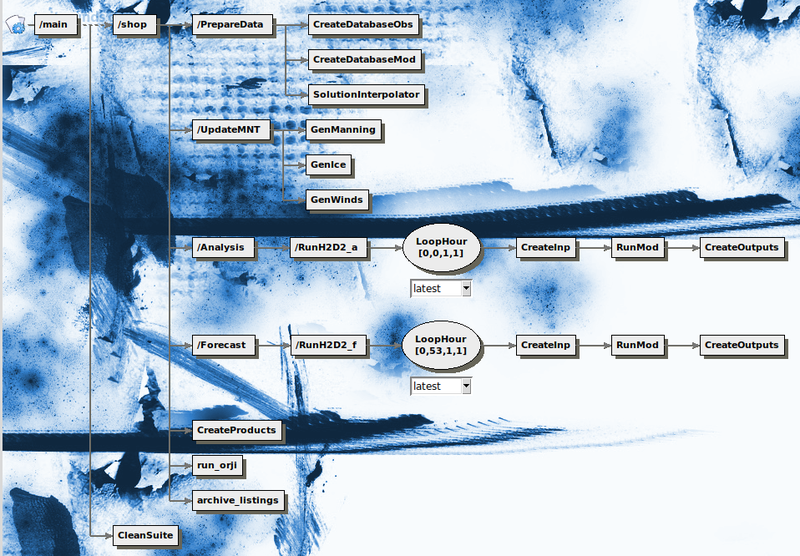
\includegraphics[scale=0.5]{800px-Flow.png}
\end{figure}

\framebreak

Main Maestro's modules under \texttt{\textcolor{blue}{/shop}} (root module)
\begin{itemize}
\item \texttt{\textcolor{blue}{/PrepareData}}:
\begin{itemize}
\item \texttt{CreateDatabaseObs}
\item \texttt{CreateDatabaseMod} 
\item \texttt{SolutionInterpolator} 
\end{itemize}
\item \texttt{\textcolor{blue}{/UpdateMNT}}: 
\begin{itemize}
\item \texttt{GenManning} 
\item \texttt{Genice}
\item \texttt{GenWinds} 
\end{itemize}

\item \texttt{\textcolor{blue}{/Analysis}} 
\item \texttt{\textcolor{blue}{/Forecast}} 
\end{itemize}
both \texttt{\textcolor{blue}{/Analysis}} and \texttt{\textcolor{blue}{/Forecast}} include this module \texttt{\textcolor{blue}{/RunH2D2}} and these tasks:\texttt{LoopHour[]} \texttt{CreateInp} \texttt{RunMod} \texttt{CreateOutputs}

Other tasks include: \texttt{CreateProducts} \texttt{CleanSuite}
\end{frame}
%-----------


%-----------
\begin{frame}[allowframebreaks]{We propose:}
Organize the code into:
\begin{itemize}
\item Pre-processing (\texttt{\textcolor{blue}{/PrepareData}}, \texttt{\textcolor{blue}{/UpdateMNT}})
\begin{itemize}
\item Data clean-up and harmonization
\item Set boundary conditions
\item \textcolor{red}{Data extraction system for multiple domains and set-ups.}
\end{itemize}

\framebreak

\item Post-processing (\texttt{CreateProducts} \texttt{CleanSuite})
\begin{itemize}
\item Data and visualization products.
\item \textcolor{red}{Conversion of output data (e.g. NetCDF)}
\item \textcolor{red}{Data validation and model assessment performance}
\item \textcolor{red}{Output data interpolation into mgrid}
\end{itemize}
\end{itemize}

\end{frame}
%-----------


%-----------
\begin{frame}{Currently working on ...}
Toolbox design for model validation and assessment of model performance:
\begin{itemize}
\item Collect, clean-up and harmonize observed data (water level, flow velocity, streamflow) at multiple locations.
\item Define performance metrics
\item Assessment of model uncertainty
\end{itemize}

\end{frame}
%-----------

\end{document}
